\chapter{Simulation Methodology}\label{app:sim_meth}

We now describe our process for conducting experiments, expanding the
outlines given in Chapters~\ref{chap:numdep},~\ref{chap:consistency},
and~\ref{chap:tempresult} demarcated into sections on evolving
relations, the consistency problem, and simulations on our temporal
logic, respectively.

\medskip

We precede this with a brief discussion of implementation issues.

\section{Notes on Implementation}\label{sec:imp_notes}


\subsection{Random Number Generation}

A number of algorithms in this thesis use randomised techniques. To
circumvent any potential problems with non-random behaviour we used
a linear congruent procedure taken
from the algorithm provided by \cite{pm88} which
avoids cycles by incorporating multiplier and modulus
having 534 million full period generators. 

\smallskip
The code was implemented in GNU C++ version 2.7.2 running
on Sun Solaris 2.5.1.  C++ with
the embedded CORAL deductive
database interface \cite{rss92} was also used for evolving relations
in Chapter~\ref{chap:numdep}. For efficiency reasons the code for procedures
described in Chapters~\ref{chap:consistency} and~\ref{chap:tempresult}
was implemented in C++ alone.

\subsection{Table Indexing}
\subsection{Code Design}




\section{Documentation of Simulations: Evolving
Relations}\label{sec:sim_er}

\subsection{

\section{Documentation of Simulations: The Consistency
Problem}\label{sec:sim_conprob}

\section{Documentation of Simulations: Numerical Dependency Temporal
Logic}\label{sec:sim_ndltl}




We now provide additional results for the consistency problem. In
Table~\ref{tbl:fd_set_used} we detail the FD sets referred to in the
following figures. All of the mean values referred to for the average
number of worlds required were obtained within batchs, each of 500
runs. The results in this appendix reinforce those presented in
Chapter~\ref{chap:consistency}.  All relations used, with respect to the
FD sets in Table~\ref{tbl:fd_set_used}, contain exactly those
attributes within the respective FD set as the schema and no more. 


{
\line
\begin{table}[ht]
\footnotesize{
\begin{center}
\begin{tabular}{|c||c||c||c||c||c||c||c|}
\hline
{\bf Set 1} & {\bf Set 2} 	& {\bf Set 4} 	& {\bf Set 6} & {\bf Set 7}	& { \bf Set 11} & {\bf Set 15}	& {\bf Set 17} \\ \hline \hline
$A \to B$ &	$A \to BC$	&  $C \to AB$	&  $D \to ABC$ & $AB \to D$ 	& $A \to B$ 	&$A \to BCD$	& $A \to B$ \\
$D \to C$ &	$D \to C$     &  $B \to AC$	&  $AB \to D$ & $D\to ABC$ 	& $D \to C$ &		& $B \to C$ \\
	&			&  		&  $A \to B$ & & $BC \to A$ &		& $C \to D$  \\
	&			&  		&  $B \to A$ & &  		&	&  \\\hline
\end{tabular}
\end{center}
}
\caption{\label{tbl:fd_set_used} FD sets used in
Figures~\ref{graph:4.3w} to~\ref{graph:histo2}}
\end{table}
}

For an FD set X $\to$ Y, where $\mid$ Y $\mid > 1$, we split this into
a set of FDs such that for all A $\in$ Y we have X $\to$ A for
expression as NDs in simulations.  This is justified given that from X
$\to^k Y$ we can infer, for all A $\in Y$, X $\to^k$ A.

\section{Average Number of Worlds Required}


We present examples showing the average number of worlds
required in batches by our chase and hill-climbing algorithm in
figures~\ref{graph:4.3w} to~\ref{graph:4.16w}.  We can see immediately
that the average number of worlds required is very small. We
hypothesise that within our random relations it is relatively easy to
generate a definite world using algorithms~\ref{alg:gen}
and~\ref{alg:chase-gen}. The average number of worlds is reduced for
larger relations with respect to a fixed domain size. Investigation
has shown this to be due to ND sets being satisfied closer to the
domain size, whilst the presence of additional tuples, with respect to
a fixed domain size, increases the number of redundant values within
indefinite cells which the chase procedure can remove. This is
particularly true of relations with larger arity indefinite cells, see
figures~\ref{graph:4.2w}, and~\ref{graph:4.13w}. Figures~\ref
{graph:4.4w} and~\ref{graph:4.12w} show this is less likely when
relations have smaller arity indefinite cells. 

\begin{figure}
\begin{minipage}{7cm}
\centerline{\scalebox{0.5}{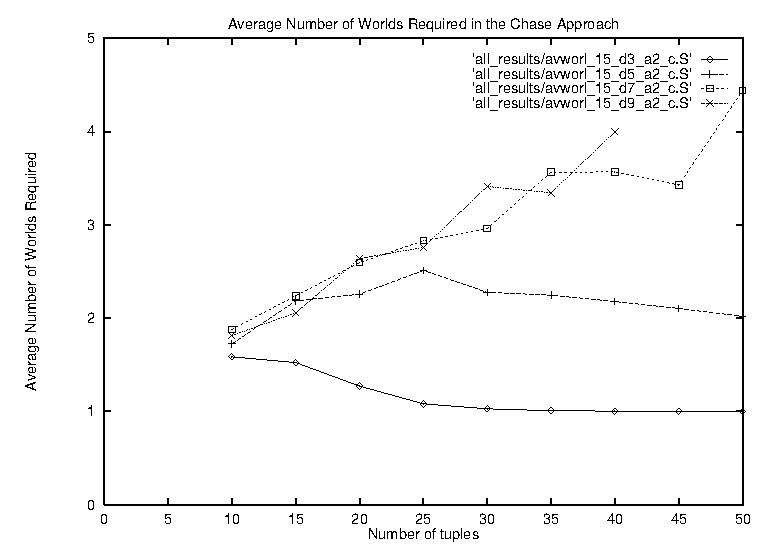
\includegraphics{../../CPP/Chase/all_results/w15_d3_a2_c.eps}}}
\caption{\label{graph:4.3w} {Average Number of Worlds Required by
the chase and hill-climbing approach for FD set 15, domain sizes 3 -
9, maximum indefinite cell arity 2 }}
\end{minipage}
\hfill
\begin{minipage}{7cm}
\centerline{\scalebox{0.5}{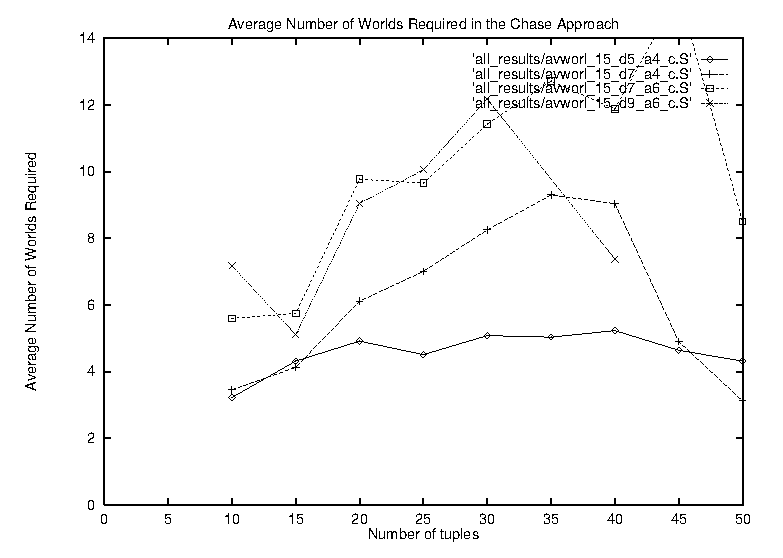
\includegraphics{../../CPP/Chase/all_results/w15_d3_a4_c.eps}}}
\caption{\label{graph:4.2w} {Average Number of Worlds
Required for FD set 15, domain sizes 5 - 9, max indefinite arity 4 - 6}}
\end{minipage}
\end{figure}

We also note that the small number of average worlds is in sharp
contrast to the number of worlds required by the naive {\em generate and
test} algorithms to obtain similar results. We are vague as to an
exact relationship due to the varying nature of both the indefinite
relations and FD sets.

\begin{figure}
\begin{minipage}{7cm}
\centerline{\scalebox{0.5}{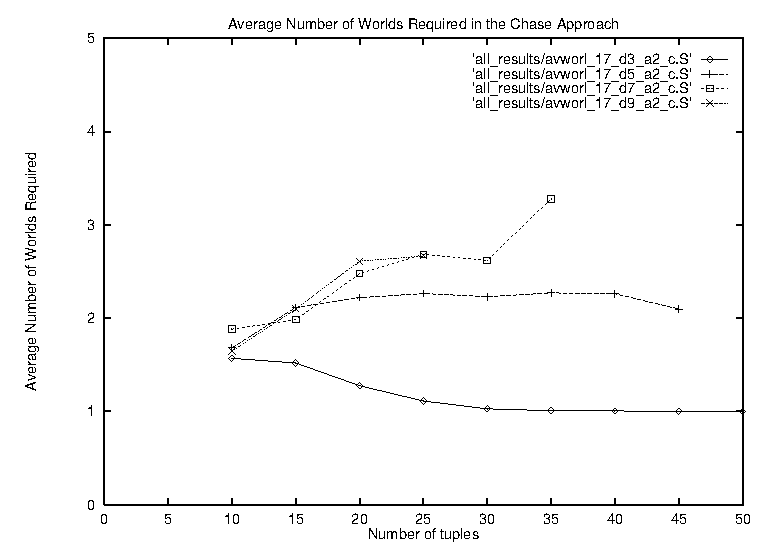
\includegraphics{../../CPP/Chase/all_results/w17_d3_a2_c.eps}}}
\caption{\label{graph:4.4w} {Average Number of Worlds
Required for FD set 17, domain sizes 3 - 9, max indefinite arity 2}}
\end{minipage}
\hfill
\begin{minipage}{7cm}
\centerline{\scalebox{0.5}{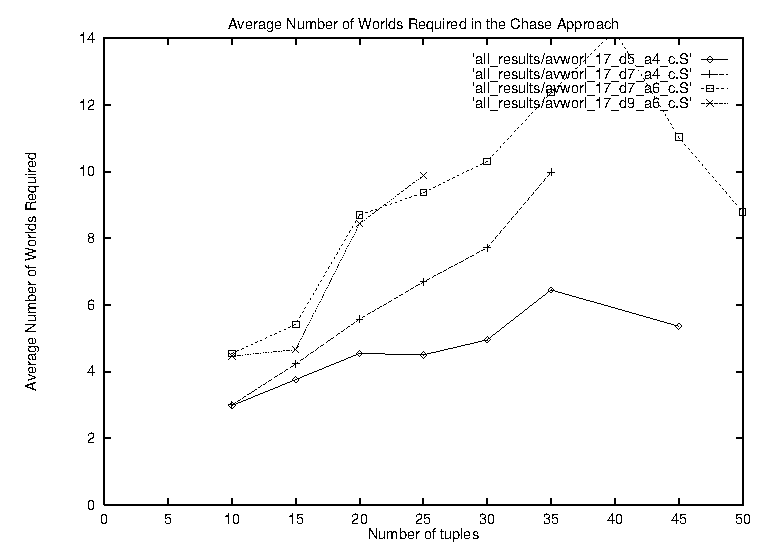
\includegraphics{../../CPP/Chase/all_results/w17_d3_a4_c.eps}}}
\caption{\label{graph:4.5w} {Average Number of Worlds Required for FD
set 17, domain sizes 5 - 9, indefinite cell arity 4 - 6}}
\end{minipage}
\end{figure}




\begin{figure}
\begin{minipage}{7cm}
\centerline{\scalebox{0.5}{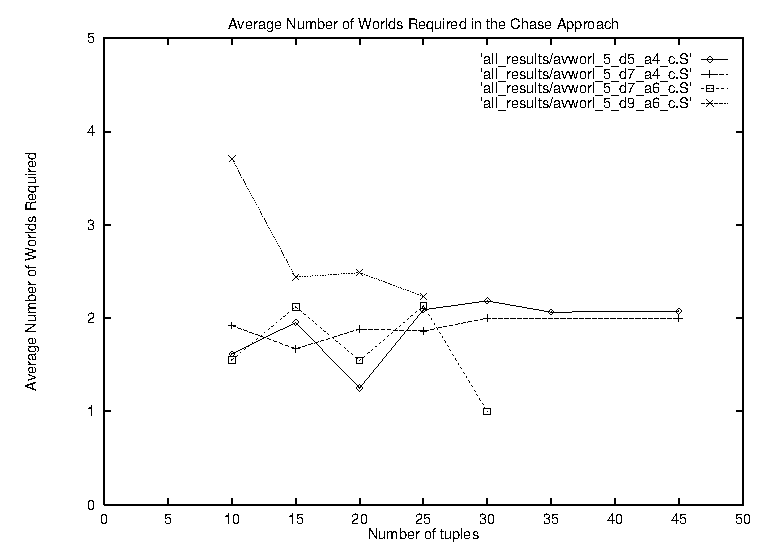
\includegraphics{../../CPP/Chase/all_results/w5_d3_a4_c.eps}}}
\caption{\label{graph:4.10w} {Average Number of Worlds
Required for FD set 5, domain size 5 - 9, indefinite cell arity 4 - 6}}
\end{minipage}
\hfill
\begin{minipage}{7cm}
\centerline{\scalebox{0.5}{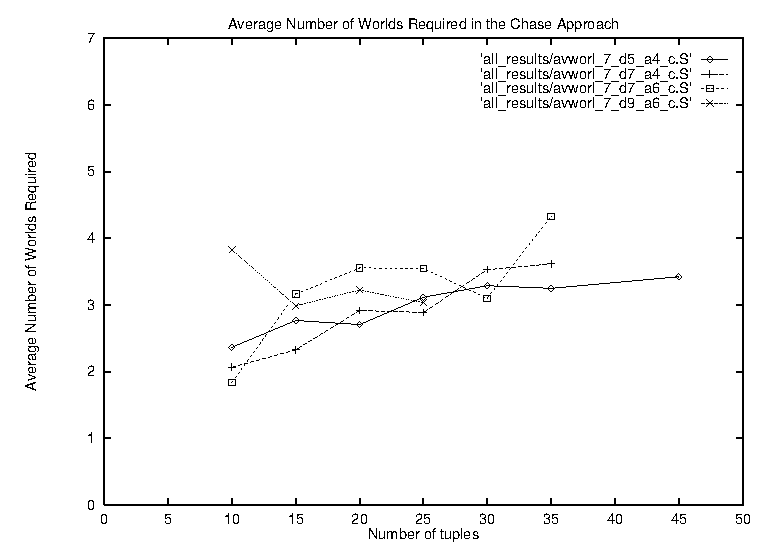
\includegraphics{../../CPP/Chase/all_results/w7_d3_a4_c.eps}}}
\caption{\label{graph:4.16w} {Average Number of Worlds
Required for FD set 7, domain size 5 - 9, indefinite cell arity 4 - 6}}
\end{minipage}
\end{figure}


\begin{figure}
\begin{minipage}{7cm}
\centerline{\scalebox{0.5}{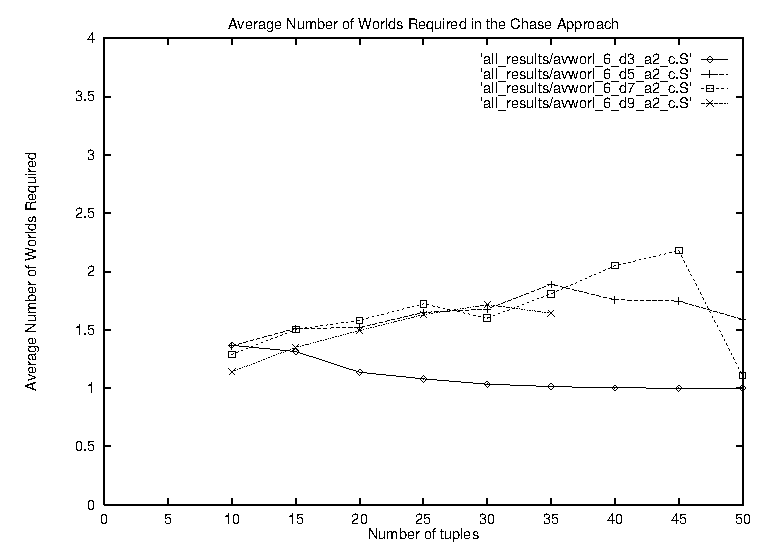
\includegraphics{../../CPP/Chase/all_results/w6_d3_a2_c.eps}}}
\caption{\label{graph:4.12w} {Average Number of Worlds
Required for FD set 6, domain size 3 - 9, indefinite arity 2}}
\end{minipage}
\hfill
\begin{minipage}{7cm}
\centerline{\scalebox{0.5}{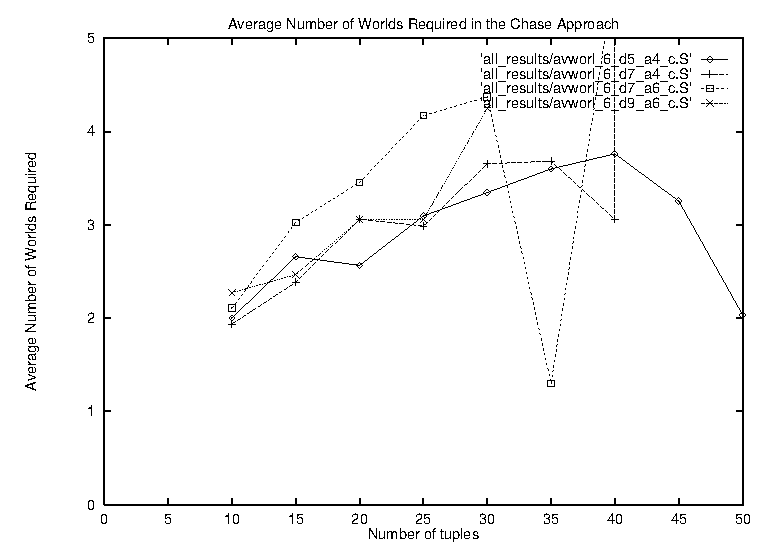
\includegraphics{../../CPP/Chase/all_results/w6_d3_a4_c.eps}}}
\caption{\label{graph:4.13w} {Average Number of Worlds required 
for FD set 6, domain size 5 - 9, indefinite arity 4 - 6}}
\end{minipage}
\end{figure}





\section{Average Proximity to FD sets}

We now discuss the proximity of our results to that of an FD set. The
increasing proximity to an FD set as relation size increases is due to
the domain size remaining fixed. Normalisation of our measure for ND
sets, a prospect for future work, would remedy this.

\medskip

We draw the following conclusions concerning proximity:
\begin{itemize}
\item On average the naive and chase procedures produce very similar
results. We emphasise that our relations were created in a uniformly
random manner. As such in the real world it may be highly likely that
a relation with indefinite information may perform better with respect
to utilising the chase and hill-climbing approach. This speculation is
enforced by the encouraging discovery that the chase procedure produce
slightly better results when a relation is sparse in indefinite cells
in arity in either attributes on the left or right hand side of
dependencies, as detailed in figures~\ref{graph:5.6}
to~\ref{graph:5.5}. 
\item Proximity to functional satisfaction increases, on average, with
an increase in the number of attributes being determined. We can see
these differences in figures~\ref{graph:6.1} and~\ref{graph:5.15}. The
difference in this case is slight but this was enforced by all
results. This is due to additional attributes being examined within
the hill-climbing process. The random nature of the relations
generated did not provide us with any pathological data
which might contradict this.
\item Whether the relation is in BCNF or non-BCNF did not, in the
data assessed, affect the results
\end{itemize}


\begin{figure}
\begin{minipage}{7cm}
\centerline{\scalebox{0.5}{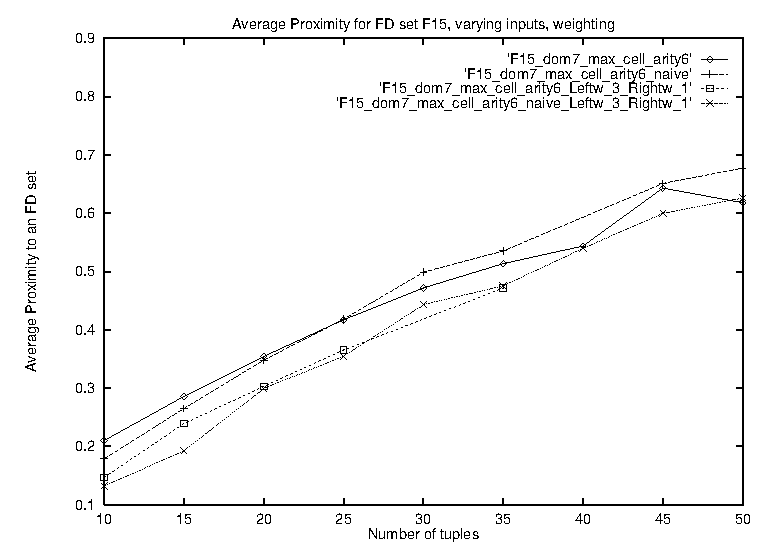
\includegraphics{../../CPP/Chase/dot_S_8_12/f15_average.eps}}}
\caption{\label{graph:5.6} {Average Proximity to FD set 15, standard
and reduced
right hand side indefinite cell weighting}}
\end{minipage}
\hfill
\begin{minipage}{7cm}
\centerline{\scalebox{0.5}{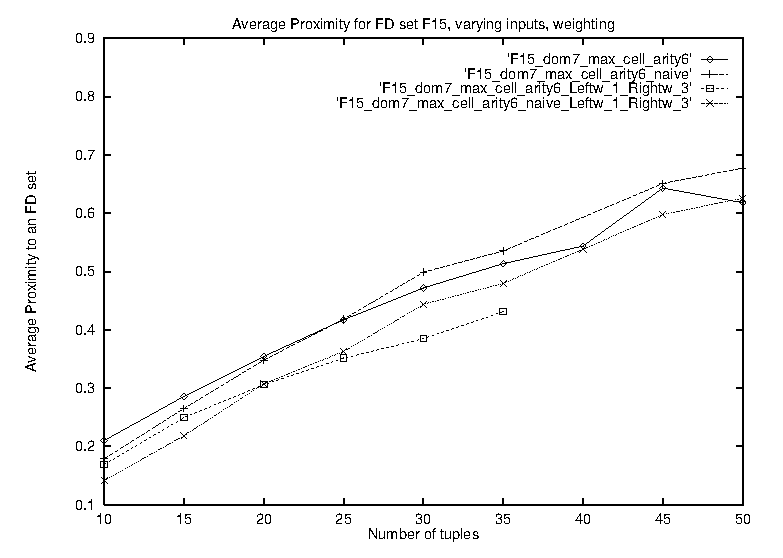
\includegraphics{../../CPP/Chase/dot_S_8_12/f15_average2.eps}}}
\caption{\label{graph:5.7} {Average Proximity to FD set 15, standard
and reduced
left hand side indefinite cell weighting}}
\end{minipage}
\end{figure}



\section{Closest Proximity to FD sets}

In contrast with the average results we find that, generally, the
best result within a batch is obtained by our chase and hill-climbing
procedure. Figures~\ref{graph:5.4} and~\ref{graph:5.5}, as well
as~\ref{graph:6.1} and~\ref{graph:5.15}, serve to emphasise that
occasionally the naive procedure, at a cost of efficiency, can
outperform the chase and hill-climbing procedure.


\begin{figure}
\begin{minipage}{7cm}
\centerline{\scalebox{0.5}{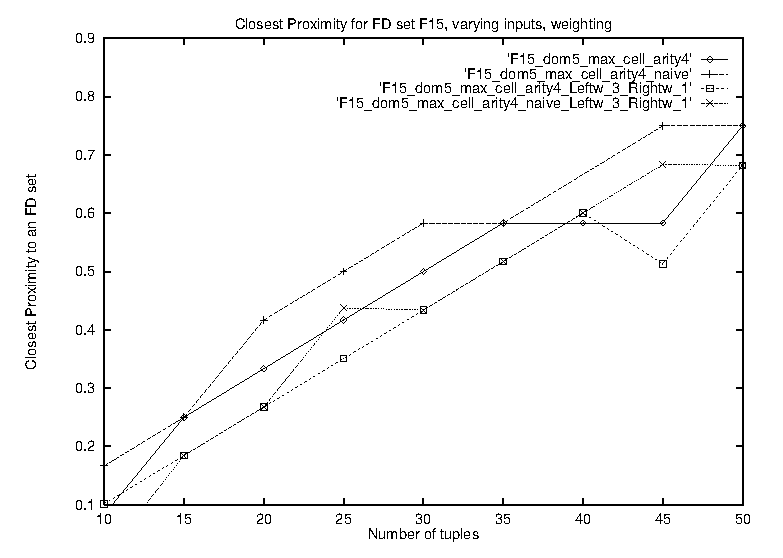
\includegraphics{../../CPP/Chase/dot_S_8_12/closest.eps}}}
\caption{\label{graph:5.4} {Closest Proximity to FD set 15 for
standard and reduced right hand side weighting of indefinite cells}}
\end{minipage}
\hfill
\begin{minipage}{7cm}
\centerline{\scalebox{0.5}{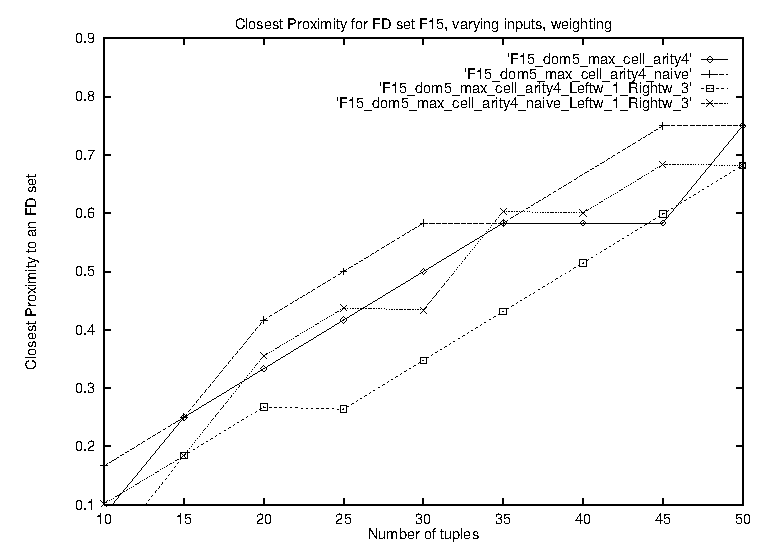
\includegraphics{../../CPP/Chase/dot_S_8_12/closest2.eps}}}
\caption{\label{graph:5.5} {Closest Proximity to FD set 15 for
standard and reduced left hand side weighting of indefinite cells }}
\end{minipage}
\end{figure}

\begin{figure}
\begin{minipage}{7cm}
\centerline{\scalebox{0.5}{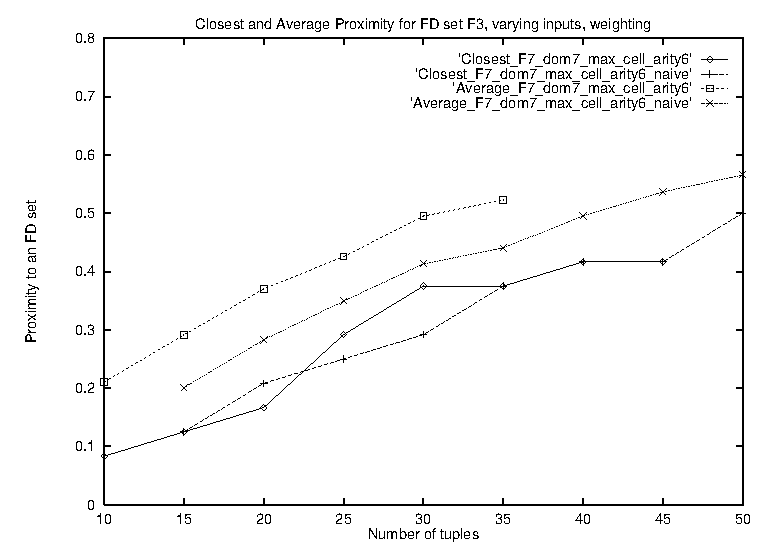
\includegraphics{../../CPP/Chase/dot_S_8_12/max2.eps}}}
\caption{\label{graph:5.13} {Average Proximity to  FD set 7, domain
size 7, max indefinite cell arity 6}}
\end{minipage}
\hfill
\begin{minipage}{7cm}
\centerline{\scalebox{0.5}{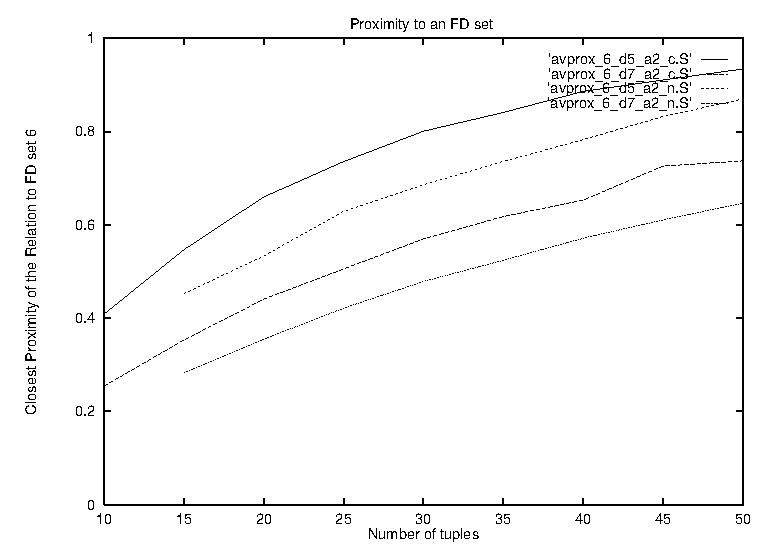
\includegraphics{../../CPP/Chase/dot_S_8_12/av6_d5_a2.eps}}}
\caption{\label{graph:5.14} {Average Proximity to FD set 6, domain
5,7, indefinite arity 2}}
\end{minipage}
\end{figure}
\newpage

\begin{figure}
\begin{minipage}{7cm}
\centerline{\scalebox{0.5}{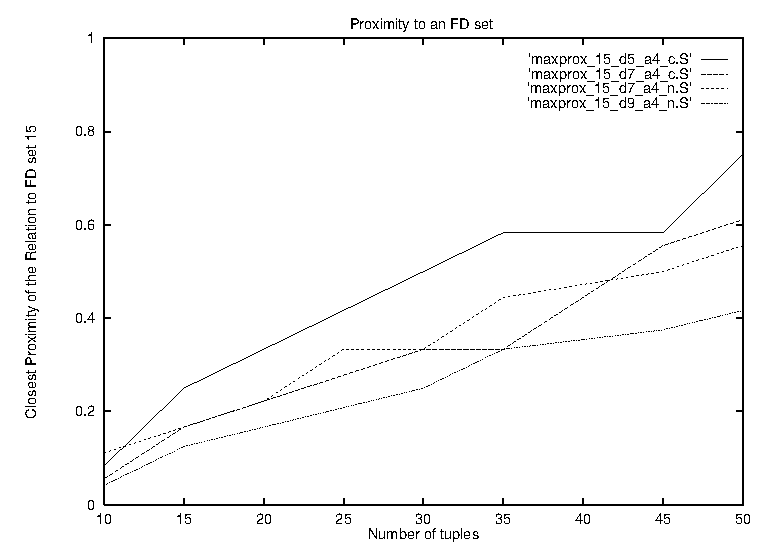
\includegraphics{../../CPP/Chase/dot_S_8_12/m15_d5_a4.eps}}}
\caption{\label{graph:6.1} {Closest Proximity to FD set 15, varying
domain sizes 5 - 9, chase and naive approaches, indefinite arity 4}}
\end{minipage}
\hfill
\begin{minipage}{7cm}
\centerline{\scalebox{0.5}{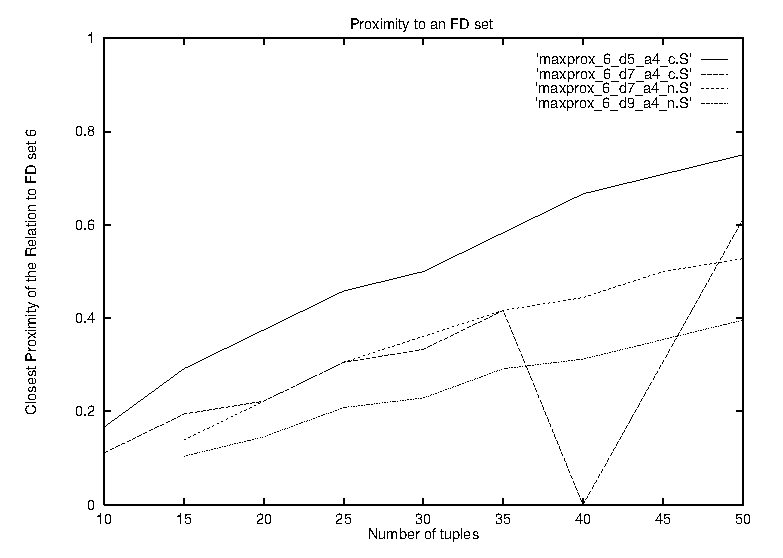
\includegraphics{../../CPP/Chase/dot_S_8_12/max6_d5_a2.eps}}}
\caption{\label{graph:5.15} {Closest Proximity to FD set 6, domain
size 5 - 9, indefinite arity 4}}
\end{minipage}
\end{figure}


\section{Jacknife and Bootstrap Comparisons}

Figures~\ref{graph:7.1}, ~\ref{graph:7.2} and~\ref{graph:7.3} present
examples of jackknife and bootstrap resampling used within our dynamic
algorithm~\ref{alg:blimit}. To ensure a fair comparison we conducted
these tests so that at each iteration each sample of possible worlds,
and therefore each sample of ND sets satisfied, was equivalent before
either bootstrap or jackknife resampling was performed. This accounts
for much of the similarity in each figure.

We draw the following conclusions:
\begin{itemize}
\item Jackknife and Bootstrap resampling will reach approximate
fixpoints, on average, at a similar number of possible
worlds. Figures~\ref{graph:7.1}, ~\ref{graph:7.2} and~\ref{graph:7.3}
are indicative of this. 
\item The jackknife resampling technique is more computationally
intensive in such a dynamic setting. The size of the bootstrap
replication is fixed, say at 50 or 100, found to be useful in this
context. \cite{et86,et93} note that sizes about 200 produce no
additional information, in general. However, the jackknife procedure
creates $n$ replicates, each of size $n-1$, when the sample size is
$n$. Therefore we have to examine 299 jackknife resamples at sample
size 300 as opposed to 100 for the bootstrap. The results show this to
be sufficient to infer a suitable standard deviation, variance, or
mean.
\item Jackknife resamples are slightly smoother due to the fact that
we are merely omitting one point in each resample. Though this may
imply it is likely to reach a fixpoint at an earlier stage, results do
not suggest this, validating, in some sense, our approach.
\end{itemize}


\begin{figure}
\begin{minipage}{7cm}
\centerline{\scalebox{0.5}{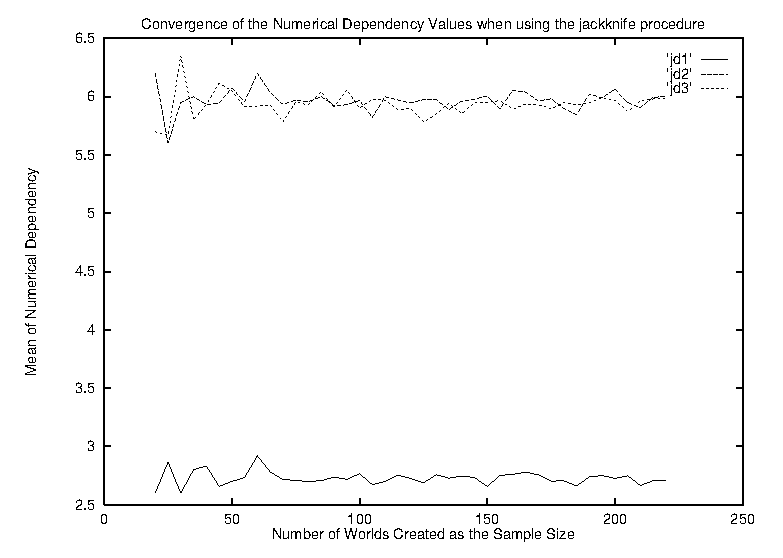
\includegraphics{../../CPP/Chase/graphs_18_2_98/jack_fd11_10_50_3.eps}}}
\end{minipage}
\hfill
\begin{minipage}{7cm}
\centerline{\scalebox{0.5}{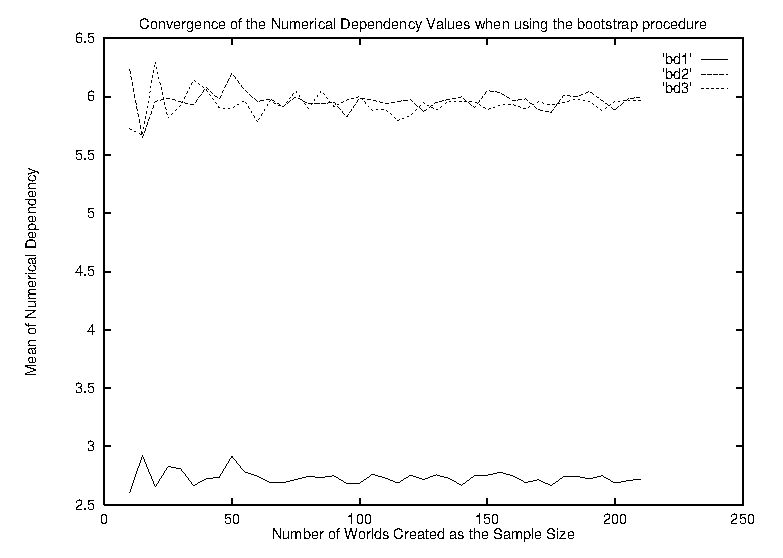
\includegraphics{../../CPP/Chase/graphs_18_2_98/boot_fd11_10_50_3.eps}}}
\end{minipage}
\caption{\label{graph:7.1} {A comparison of Jackknife and
Bootstrap mean ND set values iterated to an approximate fixpoint of
the mean using equivalent samples, for FD set 11, with a domain of 10,
50 tuples and a maximum indefinite cell arity of 3}}
\end{figure}


\begin{figure}
\begin{minipage}{7cm}
\centerline{\scalebox{0.5}{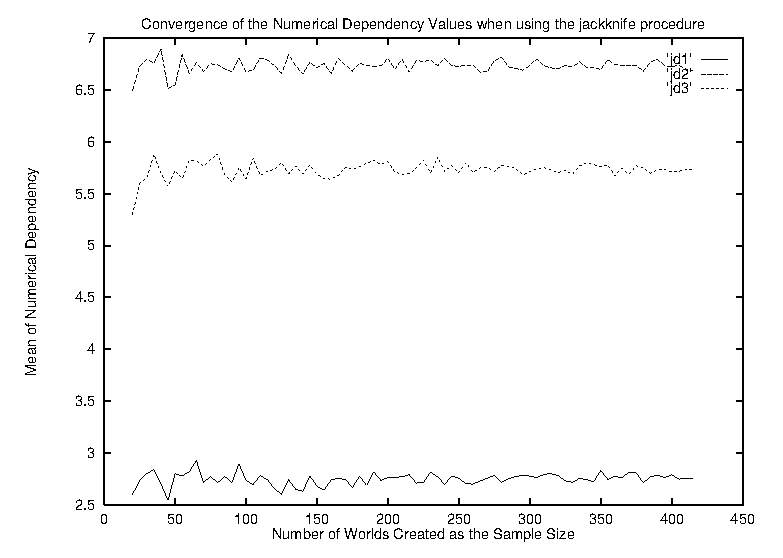
\includegraphics{../../CPP/Chase/graphs_18_2_98/jack_fd11_10_50_5.eps}}}
\end{minipage}
\hfill
\begin{minipage}{7cm}
\centerline{\scalebox{0.5}{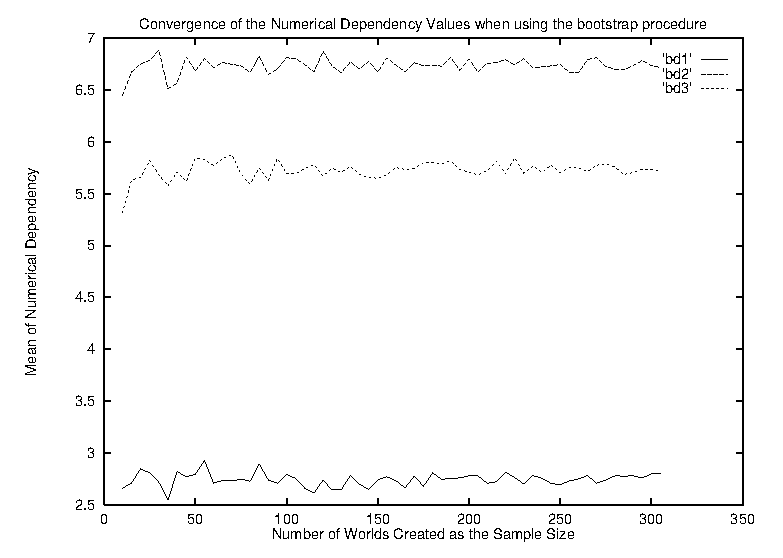
\includegraphics{../../CPP/Chase/graphs_18_2_98/boot_fd11_10_50_5.eps}}}
\end{minipage}
\caption{\label{graph:7.2} {A comparison of Jackknife and
Bootstrap mean ND set values iterated to an approximate fixpoint of
the mean using equivalent samples, for FD set 11, with a domain of 10,
50 tuples and a maximum indefinite cell arity of 5}}
\end{figure}


\begin{figure}
\begin{minipage}{7cm}
\centerline{\scalebox{0.5}{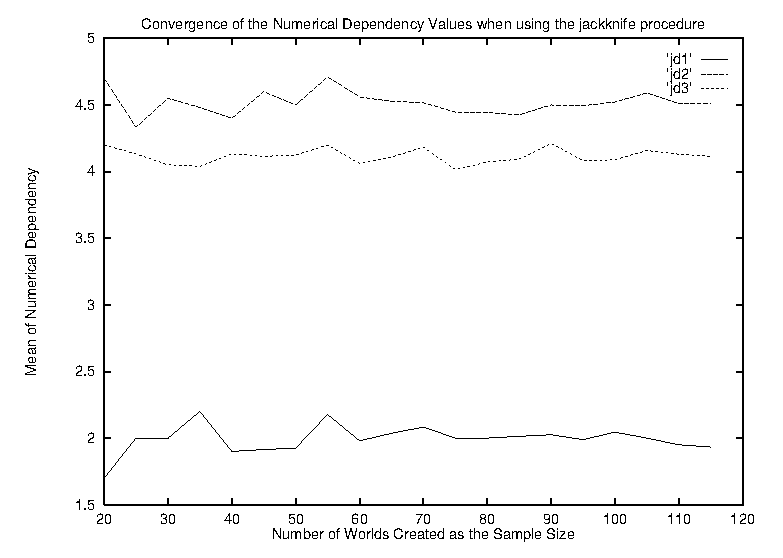
\includegraphics{../../CPP/Chase/graphs_18_2_98/jack_fd11_10_25_3.eps}}}
\end{minipage}
\hfill
\begin{minipage}{7cm}
\centerline{\scalebox{0.5}{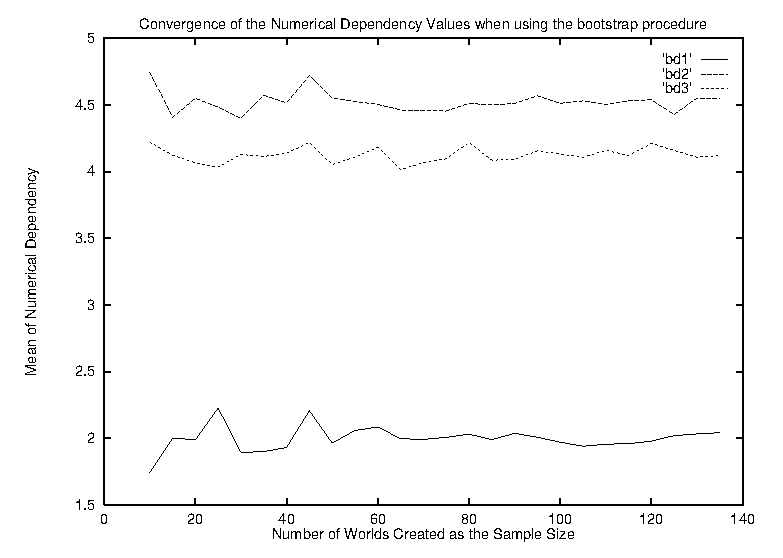
\includegraphics{../../CPP/Chase/graphs_18_2_98/boot_fd11_10_25_3.eps}}}
\end{minipage}
\caption{\label{graph:7.3} {A comparison of Jackknife and
Bootstrap mean ND set values iterated to an approximate fixpoint of
the mean using equivalent samples, for FD set 11, with a domain of 10,
25 tuples and a maximum indefinite cell arity of 3}}
\end{figure}


\begin{figure}
\begin{minipage}{7cm}
\centerline{\scalebox{0.5}{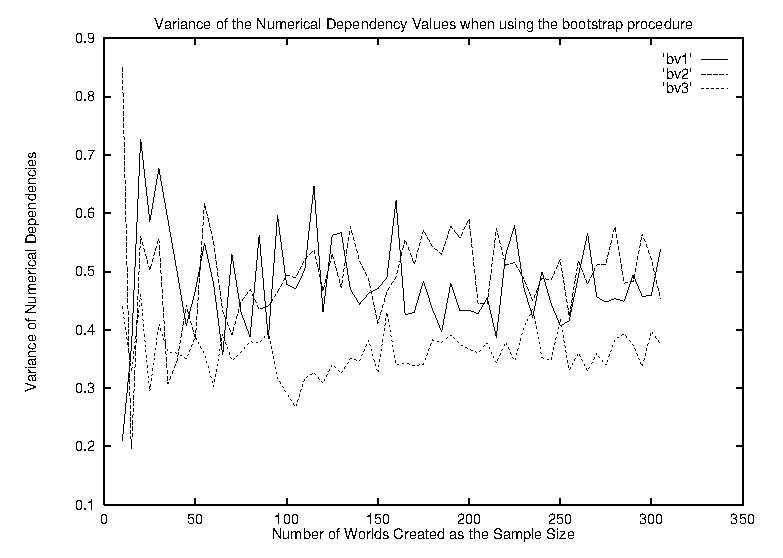
\includegraphics{../../CPP/Chase/graphs_18_2_98/boot_var_fd11_10_50_5.eps}}}
\end{minipage}
\hfill
\begin{minipage}{7cm}
\centerline{\scalebox{0.5}{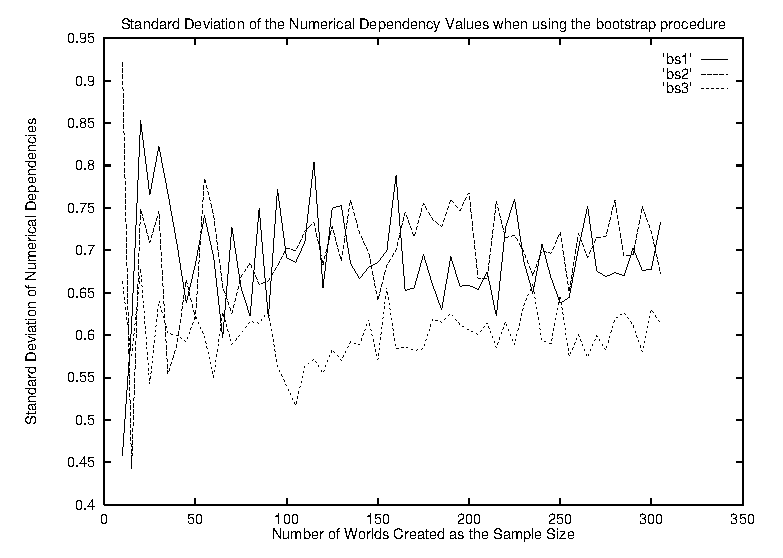
\includegraphics{../../CPP/Chase/graphs_18_2_98/boot_sd_fd11_10_50_5.eps}}}
\end{minipage}
\caption{\label{graph:7.4} {Bootstrap variance and standard deviation
convergence, for FD set 11, with a domain of 10, 25 tuples and a maximum indefinite cell arity of 3}}
\end{figure}


Figure~\ref{graph:7.4} highlights convergence of the standard
deviation and variance as the sample size is increased. We are dealing
with approximate fixpoint and this implies equality within confidence
limits shown in Figure~\ref{graph:conlim}. 

\subsection{Bootstrap Variance Results}

\begin{figure}
\begin{minipage}{7cm}
\centerline{\scalebox{0.5}{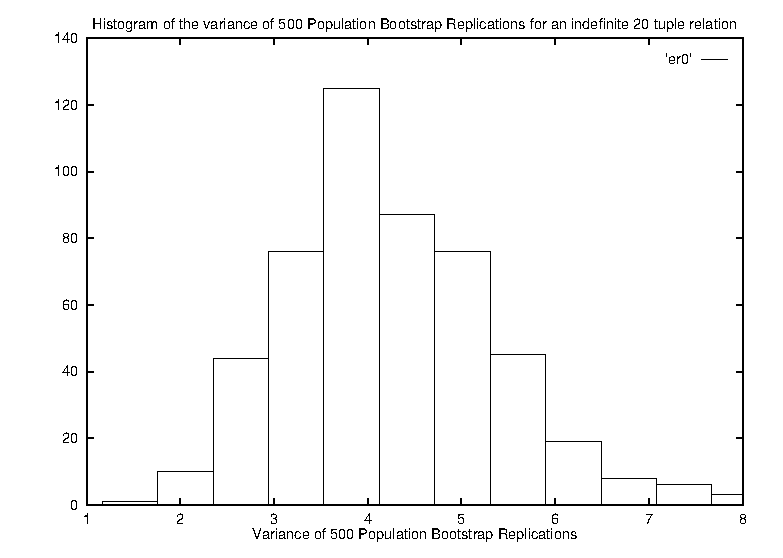
\includegraphics{../../CPP/Chase/all_results/var2500.eps}}}
\end{minipage}
\hfill
\begin{minipage}{7cm}
\centerline{\scalebox{0.5}{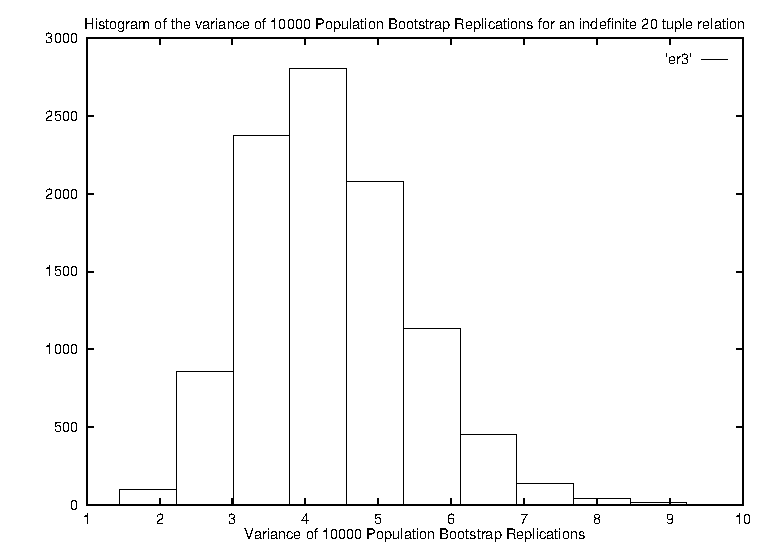
\includegraphics{../../CPP/Chase/all_results/var210000.eps}}}
\end{minipage}
\caption{\label{graph:histo2} {Histograms displaying variance of 500 and 10000 bootstrap replications}}
\end{figure}

Figure~\ref{graph:histo2} display the overall similarity in variances
achieved for 500 and 10000 BRS, respectively, complementing
Figure~\ref{graph:cp_hist1}.


